\chapter{Analysis}
\label{chap:analysis}

This chapter starts in section \ref{sec:parti_analysisbird} with an analysis of the proposed reconstruction-based random projection method under varying parameter settings. Section \ref{sec:parti_final} shows the performance under fixed parameter settings in comparison with the baseline. Finally some concluding remarks are provided in section \ref{sec:parti_concluding}.


\section{Analysis methodology}
\label{sec:analysis_methodology}
\subsection{Data}
First analysis on artificial data, then in chapter 6 we continue with a real-world data set. We take an artificial data set first, as we want to analyse our approaches under varying settings. We also want to make sure we do not penalize the methods in case they do not flag a data point that does not deviate from the remaining data points based on its representation by the available data but is labelled as being an outlier, or in case they do find a data point that deviates significantly from other data points but which is not labelled as being an outlier. Such situations are interesting to study further, but require domain specific knowledge and we do not want to adapt our analysis to a specific domain. In section \ref{chap:experiments} we assess the approaches in real-world settings using publicly available data sets.\\

EXPLAIN ARTIFICIAL DATA HERE\\

Two random subsets of 20\% of the 60 time series were imputed with either point or collective outliers. 

EXPLAIN WINDOW FUNCTION\\


\subsection{Performance metrics}

\subsubsection{Detection performance}
In the ideal scenario we would detect all outliers, and flag no data points belonging to the `normal' class as outlier. This perfect scenario is often not realistic and therefore we need to find a balance between incorrectly labelling outliers as normal data points and vice versa. In this thesis, outliers are generally considered as the positive class, where normal data points are referred to as belonging to the negative class. In case an outlier is correctly labelled as being positive, we refer to that as a true positive (TP). In case it is mislabelled we say it is a false negative (FN). For normal data points this works the opposite direction. The balance between labelling positives correctly and negatives incorrectly can be reflected by many different metrics. Two such metrics are the FP-rate \eqref{eq:fp-rate} and TP-rate \eqref{eq:tp-rate} which are important for outlier analysis \cite{aggarwal2015outlier}. 

\begin{equation}
\label{eq:tp-rate}
TP = \frac{TP}{TP}
\end{equation}

\begin{equation}
\label{eq:fp-rate}
FP = \frac{FP}{FP}
\end{equation}

We have chosen to use the Receiver Operator Statistic (ROC) and its corresponding Area Under the Curve (AUC) to evaluate the effectiveness of our outlier detection method.

[The ROC blablabla, operating point different threshold, state number of thresholds (depends on the number of data points). The AUC... EXPLAIN, show a figure or not, but at least explain how it should be interpreted].
The AUC is said to reflect the probability of a randomly selected pair of data points, of which each belongs to the opposite class, will be correctly classified in the sense that the outlier is assigned with a higher probability of being an outlier and vice versa \cite{hanley1982meaning}. Therefore, the AUC can guide the interpretation of the ROCs.


The disadvantage of evaluating the performance with the ROC and corresponding AUC, is that each operating point is based on the same threshold for all outlier scores and thus data points. This possibly yields a biased reflection of the actual detection performance \cite{mchugh2000testing}. That is, the actual threshold cannot be learned from the data on forehand and would probably be adaptive in our problem context. The thresholding method is considered beyond the scope of this thesis but adaptive threshold options are available in the literature. An often used threshold is the 3-sigma rule which assumes outliers to have a distance of 3 standard deviations from the average \cite{zimek2012survey}. We will closely inspect the results of the detection methods before any threshold is applied by observing the outlier scores.

An alternative would be to replace the ROC curve with the Precision-Recall curve, but this curve is less intuitive to interpret and is considered not superior to the ROC for the evaluation of outlier detection methods \cite{aggarwal2015outlier}.\\

As we do not focus this analysis on any specific application, we consider both types of misclassifications as having the same impact and therefore we take the misclassificaton costs as being equal.



\subsubsection{Computational efficiency}
The second metric we want to analyse our methods with is its runtime performance. As often time series analysis is in on-line or streaming mode (elaborate).

In comparison to each other, as we do not .



\subsubsection{Memory efficiency}
The second metric we want to analyse our methods with is its runtime performance. As often time series analysis is in on-line or streaming mode (elaborate).

In comparison to each other, as we will not .


%Before we continue, it is important to first answer the question whether it improves our detection performance if we scale back the distances with $\sqrt{\frac{d}{k}}$ to preserve the original distances. Table \ref{tab:back-scaling} shows the average and standard deviation of the AUCs of the unscaled and scaled implementations with $k=50$ for 50 successive runs.
%
%\begin{table}[h]
%	\centering
%	\caption{Detection performance random projection method with and without back-scaling by factor $\sqrt{\frac{d}{k}}$ over 50 runs.}
%	\begin{tabular}{l  c  }
%		\toprule
%		Scaling setup			&	AUC 				 \\ \midrule
%		With back-scaling		&	0.8575 (\pm 0.0460)  \\
%		Without back-scaling	&	0.8933	(\pm 0.0147) \\ \bottomrule
%	\end{tabular}
%\end{table}
%
%If we look at the performances of each run in figure \ref{fig:back-scaling}, it seems that scaling back the projected vectors with $\sqrt{\frac{d}{k}}$ on average performs worse. A significant number  of runs (40/50) without scaling back the projected vectors yields a higher AUC. Finally, as was illustrated already by the difference in standard deviation, the performance without back-scaling is much more stable than its counterpart.
%
%\begin{figure}[h]
%	\centering
%	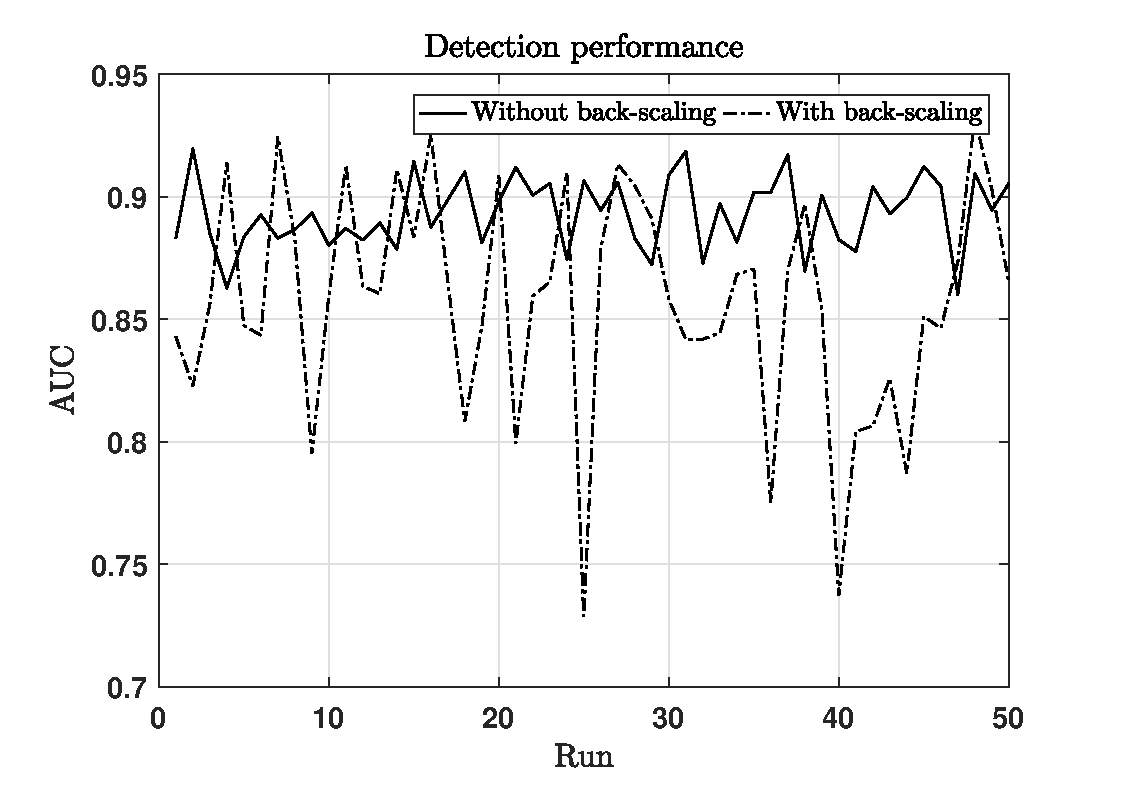
\includegraphics[scale=0.4]{parti/AUCs_backscaling}
%	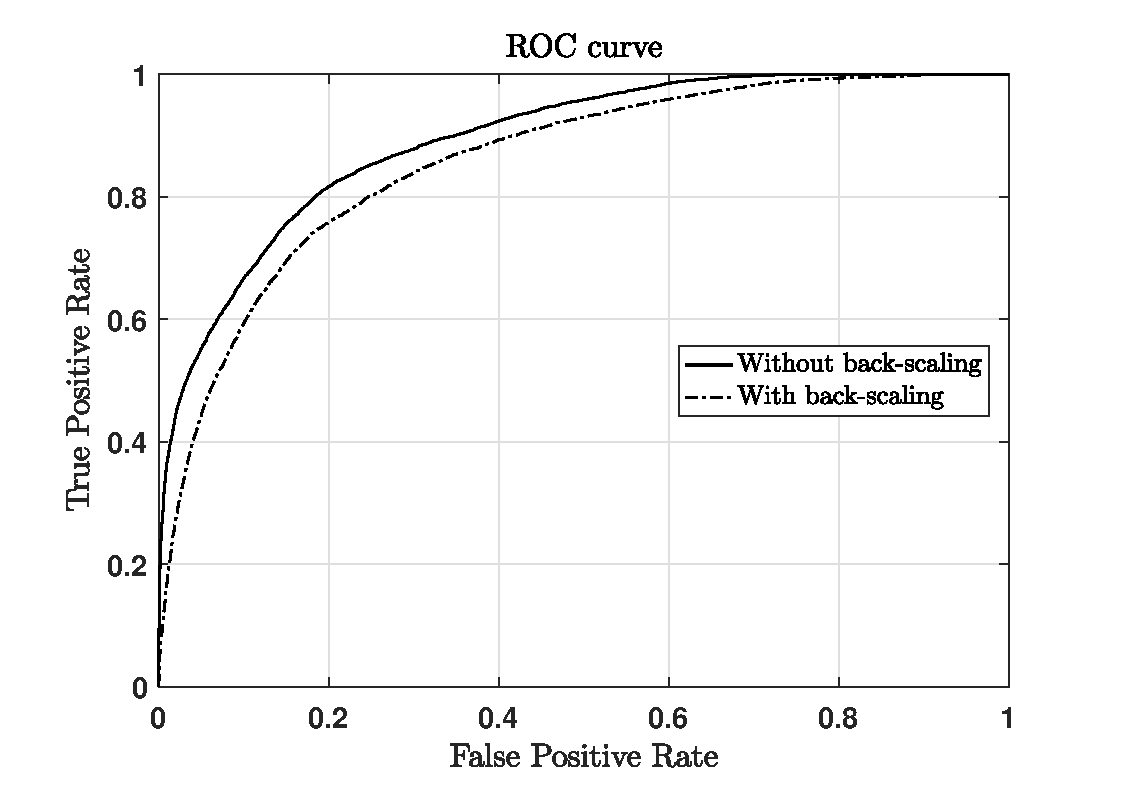
\includegraphics[scale=0.4]{parti/Avg_ROC_backscaling}
%	\caption{AUCs over 50 runs and average ROCs of the random projection implementations with and without back-scaling.}
%	\label{fig:back-scaling}
%\end{figure}

\section{A bird's-eye view}
\label{sec:parti_analysisbird}
%What we want to get out of here is an impression of the potential of the methods, and the overall strengths and weaknesses, without zooming in on the specific performance given a fixed set of parameters.

[Results in full dimensionality etcetera to provide full insights in the course of the runtimes of both approaches, and also show the sensitivity of the number of components (i.e. it might make a large difference when setting the `energy' to be explained ranging from 0.95 to 0.999 as one component more or less heavily impacts the total performance. That is, we want to find the outliers specifically so it's crucial here to not model those in our principal component, we are likely better off explaining too little variance than too much.)]\\

Having investigated the random projection method for reconstruction-based outlier detection, we continue with an analysis of the method in comparison with the baseline SPIRIT. For these experiments we make use of the original data set of $d=60$ and expand it with the window function using window lengths $5, 10 \text{ and } 15$. The AUCs are generated by fixing $k$ to a value ranging from 1 to 50. SPIRIT can however be deployed adaptively adjusting $k$ on-line, so the results for fixing $k$ would be most interesting for applications where we actually have prior knowledge available to derive the number of components from.

While SPIRIT is deterministic, the proposed method based on random projections is not. Therefore, the AUC scores of the latter are averaged over 10 runs. The runtime of both methods is also being averaged over 10 runs. Figures \ref{fig:parti_AUCs} and \ref{fig:parti_runtimes} show the results of these experiments.

\begin{figure}[h]
	\centering
	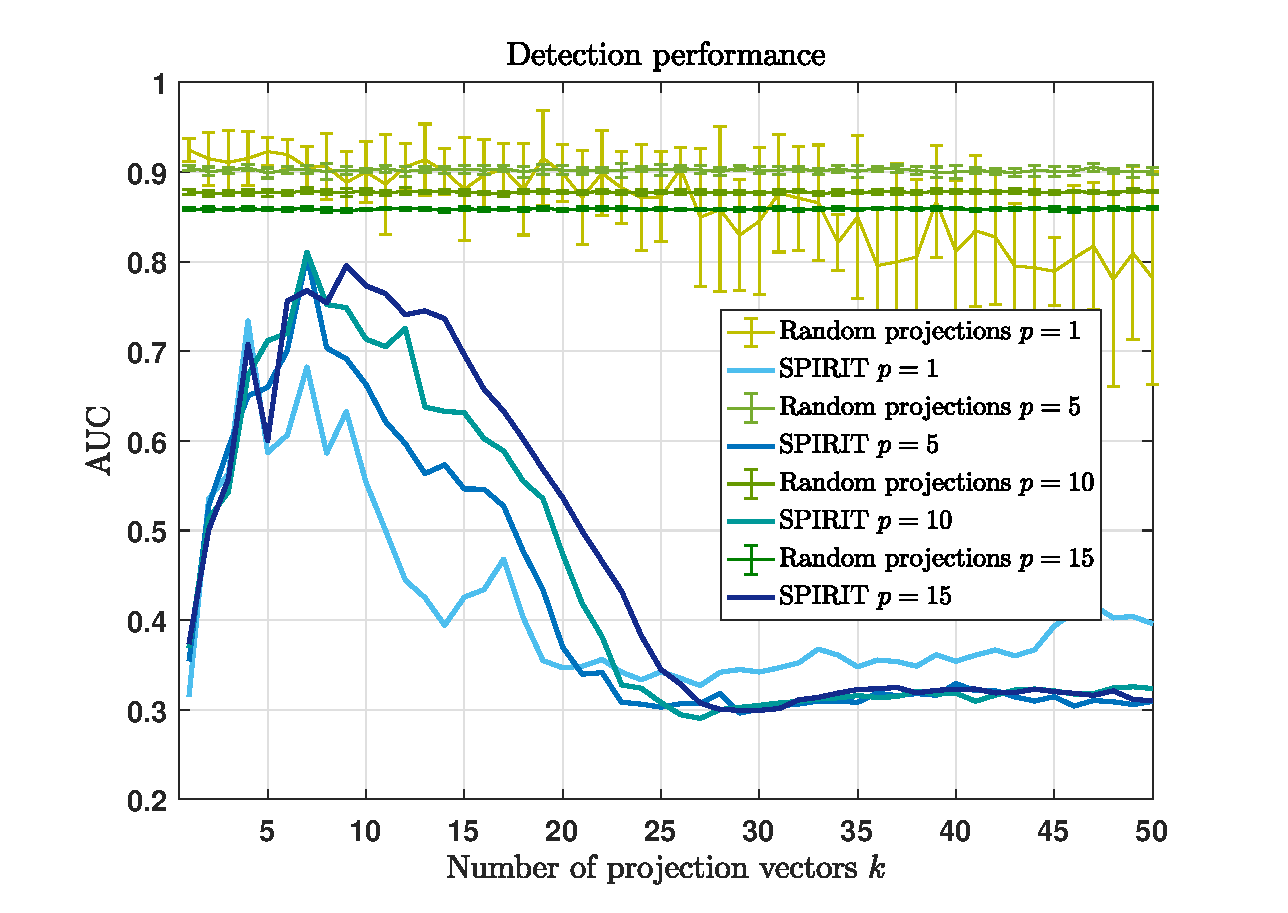
\includegraphics[scale=0.5]{parti/AUCs}
	\caption{AUC of the random projection method and SPIRIT for window length $p={5,10,15}$ resulting in $d={300,600,900}$ with $k$ ranging from 1 to 50.}
	\label{fig:parti_AUCs}
\end{figure}

\begin{figure}[h]
	\centering
	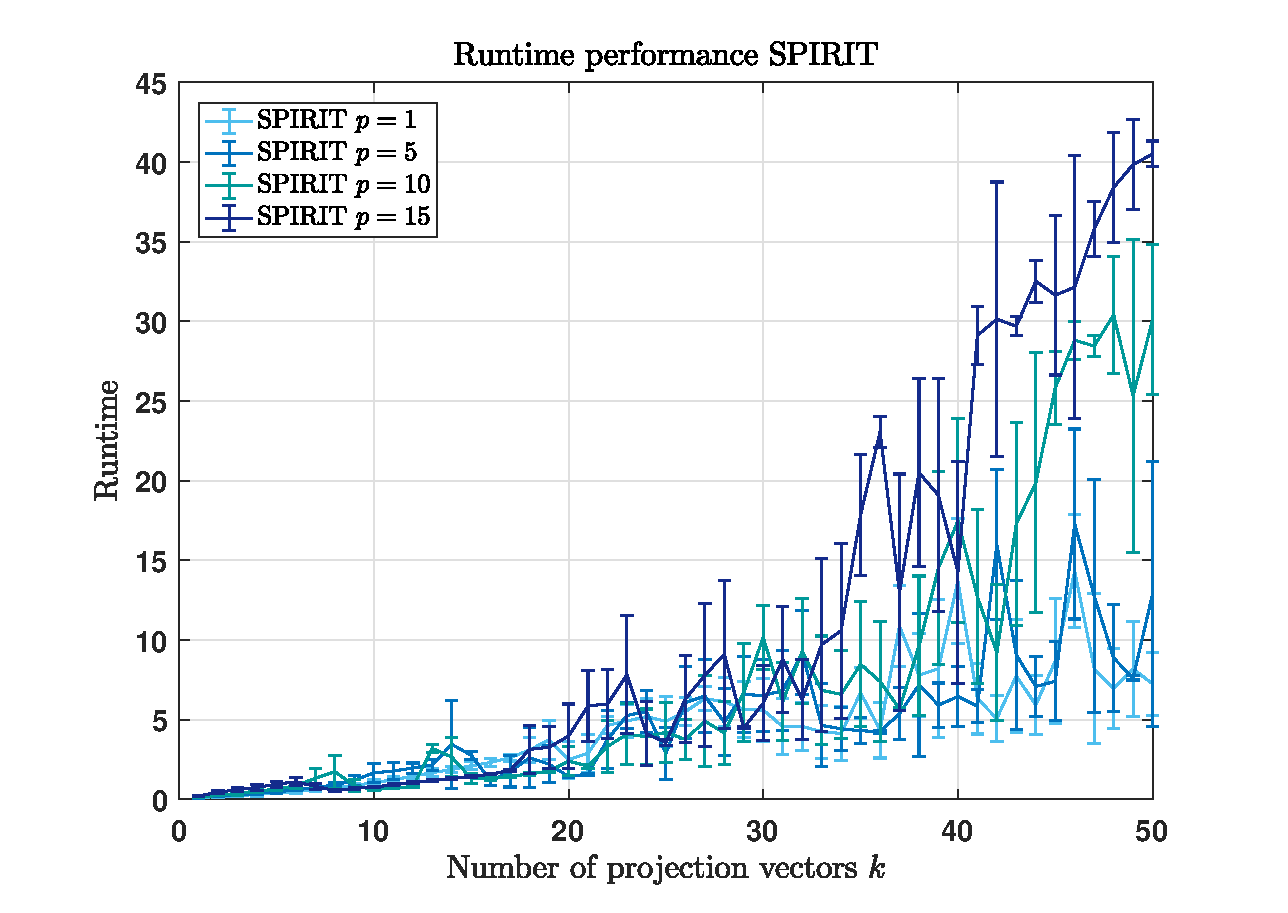
\includegraphics[scale=0.4]{parti/runtimes_SPIRIT}
	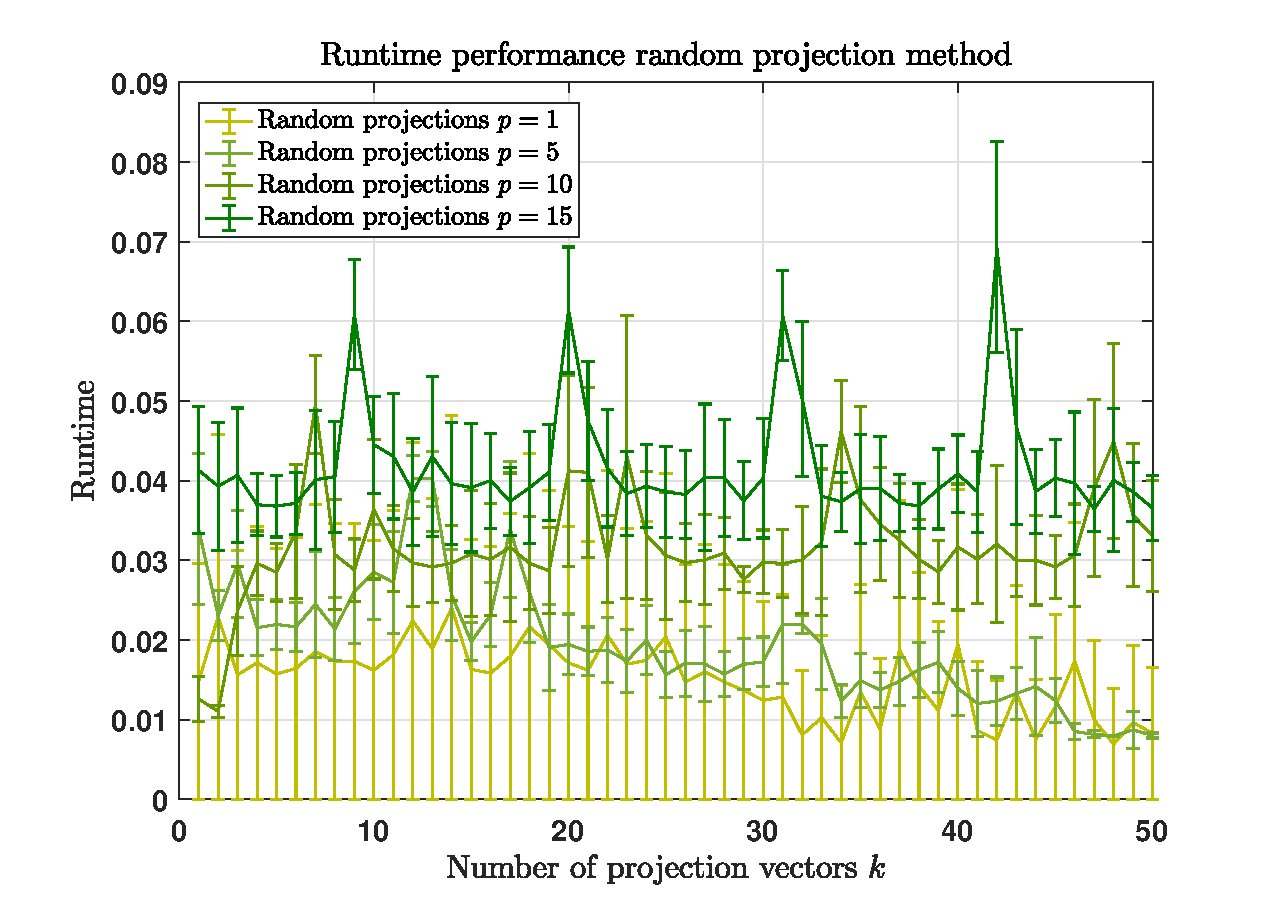
\includegraphics[scale=0.4]{parti/runtimes_RP}
	\caption{Runtime performances of the random projection method and SPIRIT for window length $p={5,10,15}$ resulting in $d={300,600,900}$ with $k$ ranging from 1 to 50.}
	\label{fig:parti_runtimes}
\end{figure}


[Give more insights: interpret runtime, detection performance, $k$ sensitivity]\\

From these results it could be concluded that the proposed method performs very well, based on this artificial data set and considering these performance metrics. The proposed method requires a small window length as its detection and runtime performances are best for $p=5$, where the influence of the number of projection vectors $k$ shows only little decrease in average AUC over a large range. 

The random projection method performs remarkably well with only very few projection vectors, i.e. reconstructing the data from a very low-dimensional projection. It sounds odd that we can reconstruct our data by projecting all data points in only one random direction. And the intuition is that such a projection indeed results in a very poor reconstruction of the normal data points. 
It might be questioned how it can possibly make the outliers still reasonably observable by reconstruction-based detection? Our thought on this, is that the outliers get reconstructed even more poorly than the normal data points, which would then explain the higher reconstruction error. 
Following this reasoning, it would also make sense that adding projection vectors from some point only makes the performance worse. Possibly the reconstruction quality of the outliers is improving with a higher rate than the reconstruction quality of the normal data points. 

Another factor that could play a role here, is that we are looking at the data points in relation to each other over time. The lemma guarantees distance preservation from some projection dimension $k$ which depends logarithmic on the number of data points $n$ between which the pair-wise distances are desired to be preserved. In our stream of data, it might be sufficient to aim for pair-wise distance preservation over a smaller window of data points.\\


However, as we are comparing it to an on-line principal component approximation method, one might also get the idea that the on-line principal component estimation method is an `unfair' comparison. In order to make the comparison a bit harder, we have conducted outlier detection using an off-line principal component analysis method as well. This method optimizes the coefficients over the entire data set instead of just the history up to a certain time step\footnote{Recall that this does not meet the conditions of the context we are studying. It is merely giving an idea of the potential of the general principal component method.}. 

The off-line principal component analysis reconstruction-based outlier detection method yields a detection performance of 0.8919, requiring a window length of $p=15$ and 41 components to explain a fraction of 0.997 of variance. This off-line method is just like the on-line version very sensitive to small changes in this last parameter, which makes it unlikely that this performance will generalize well to unseen data sets. Despite the optimization of off-line PCA on the full data set, and fine-tuning the fraction of variance explained by the components, it still performs worse than the proposed random projection method. 


%We would like to remark that it has a high impact on the performance of the random projection method if we do not scale the projected vectors back with the scaling factor $\sqrt{\frac{d}{k}}$ as was already illustrated by figure \ref{fig:back-scaling}. 


\section{Final decisions?}

To observe the performance of the methods more closely, we will provide insights in what is actually being detected, and what not. To do so, we look at the ROC curves of the baseline SPIRIT, the off-line PCA method and the random projection method. Recall that the off-line PCA method was allowed for optimization of the coefficients over the entire data set, where we also heavily fine-tuned the fraction of variance being explained by the components. In contrast, the baseline method (adaptive) SPIRIT approximates the number of principal components needed to explain most of the variance on-line, but also requires lower and upper bounds that guide this on-line adaptation of the number of components. An alternative option considered is to fix the number of components and let SPIRIT update the coefficients (corresponding to the fixed number of components) on-line. Finally, SPIRIT requires a forgetting factor $\lambda$ which is taken to be 0.97 as within the suggested range 0.96 - 0.98 \cite{papadimitriou2005streaming}. Additional parameters that play a role are the window size having an impact on all methods, and $\lambda$ for SPIRIT in specific. 

We would be cheating if we would evaluate the proposed method by taking the observed best value for the number of projection vectors $k$ from the AUC curve in figure \ref{fig:parti_AUCs}. Therefore we compute the performance regarding the $TPR$ and $FPR$ for all operating points over a range for $k$ from 1 to 8, averaged over 50 runs. This way, we believe that we obtain the most realistic view on the performance of the proposed method. Table \ref{tab:parti_characteristics} summarizes the characteristics (parameters, AUC and runtime performance) associated with the model(s) used for generating the ROC curves in figure \ref{fig:parti_rocs}. The runtime of the principal component based methods is averaged over 10 runs.\\

[ADD WINDOW SIZE!!]\\

\begin{table}[h]
	\centering
	\caption{Performance under fixed parameters}
	\label{tab:parti_characteristics}
	\begin{tabular}{l c c c c}
		\toprule	
		Method				& Parameter			& Value		&	AUC	& Runtime\\
		\midrule
		Adaptive SPIRIT		& $\lambda$			&	0.97	& 0.917	& 1.654 (\pm 0.493) \\
							& Variance bounds	&	[0.99 0.998] & 	& \\		
		Fixed SPIRIT		& $\lambda$			&	0.97		& 0.810 & 1.089 (\pm 0.133)\\
							& $k$				&	7			& & \\
							& $p$				&	10		&		&\\
		Off-line PCA		& Variance bound	&	0.997	& 0.892 & 1.009 (\pm 0.198)\\
							& $p$				&	15		&		&\\
		Random projections	& $k$				&	1		&	0.928 (\pm 0.011) & 0.024 (\pm 0.004)\\
		\bottomrule
	\end{tabular}
\end{table}


\begin{figure}[h]
	\centering
	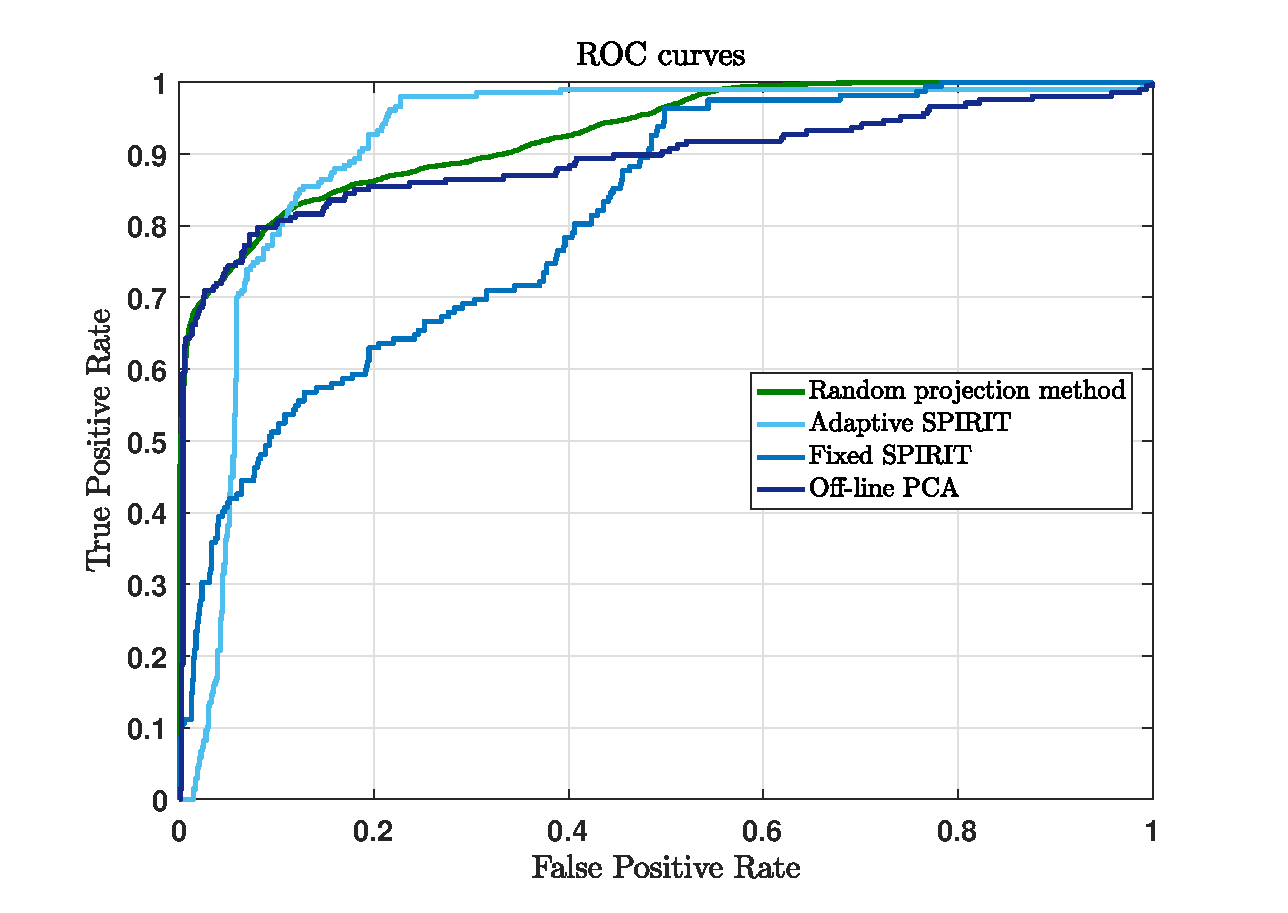
\includegraphics[scale=0.5]{parti/ROCs}
	\caption{ROC curves of the optimized off-line PCA and SPIRIT, and the random projection method $k=1$ over 50 runs.}
	\label{fig:parti_rocs}
\end{figure}

Despite its better performance, deploying the random projection method on the not expanded data set results in a higher standard deviation AUC-wise. This observation implies that taking a combination of outlier detectors using the low-cost random projection method would lower this standard deviation. We experimented with this as well, and taking for instance 10 distinct predictions yields an average AUC of 0.929 and reduces the standard deviation very close to 0.

[INTERPRET ROCs!!! Check the pros and cons of the false positives versus true positives etc.]\\

As became clear in section \ref{sec:parti_analysisbird} the Adaptive SPIRIT approach is very sensitive to changes in the variance bounds. Taking a range of [0.99 - 0.995] makes the AUC drop to 0.751 and [0.98 - 0.99] results in an AUC of 0.672. 

To move away from thresholds, figure \ref{fig:parti_outlierscores} shows the outlier scores as generated by the models corresponding to the ROC curves in figure \ref{fig:parti_rocs} and characteristics in table \ref{tab:parti_characteristics}. For the random projection method the output of the last run associated with an AUC of 0.930 is shown. Note that the reconstruction errors of the random projection method are significantly higher as we do not scale the projected vectors back to preserve the pair-wise distances or vector norms. This results in a larger difference between the reconstructed vector and the original one, which then causes a higher reconstruction error and outlier score. 

The difference in darkness of the outlier scores generated by the principal component based outlier detection (in blue) is proportional to the amount of prior knowledge, or supervision, needed to obtain the results. 

\begin{figure}[h]
	\centering
	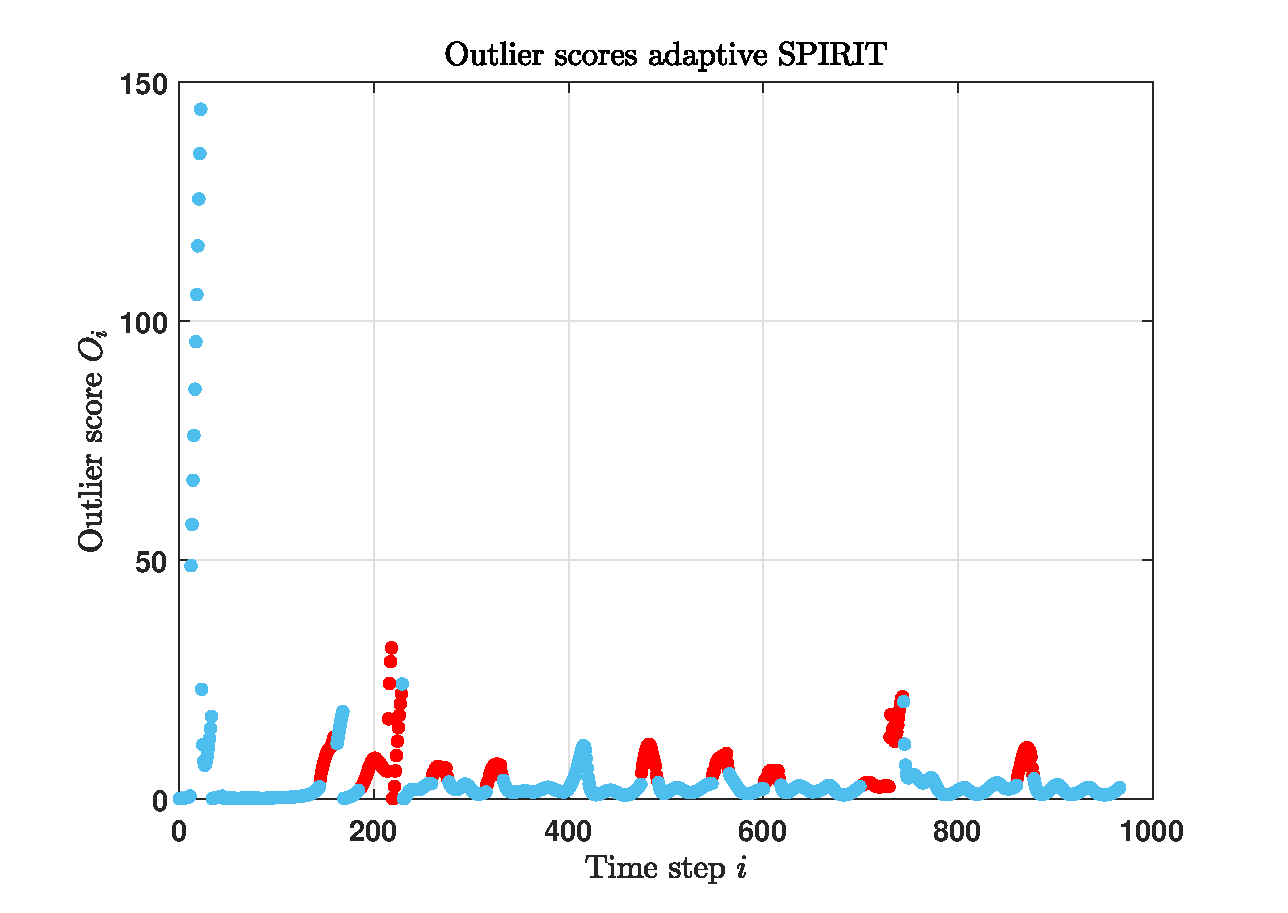
\includegraphics[scale=0.3]{parti/Outlierscores_adaptiveSPIRIT}
	\label{fig:parti_outlierscores_adaptivespirit}
	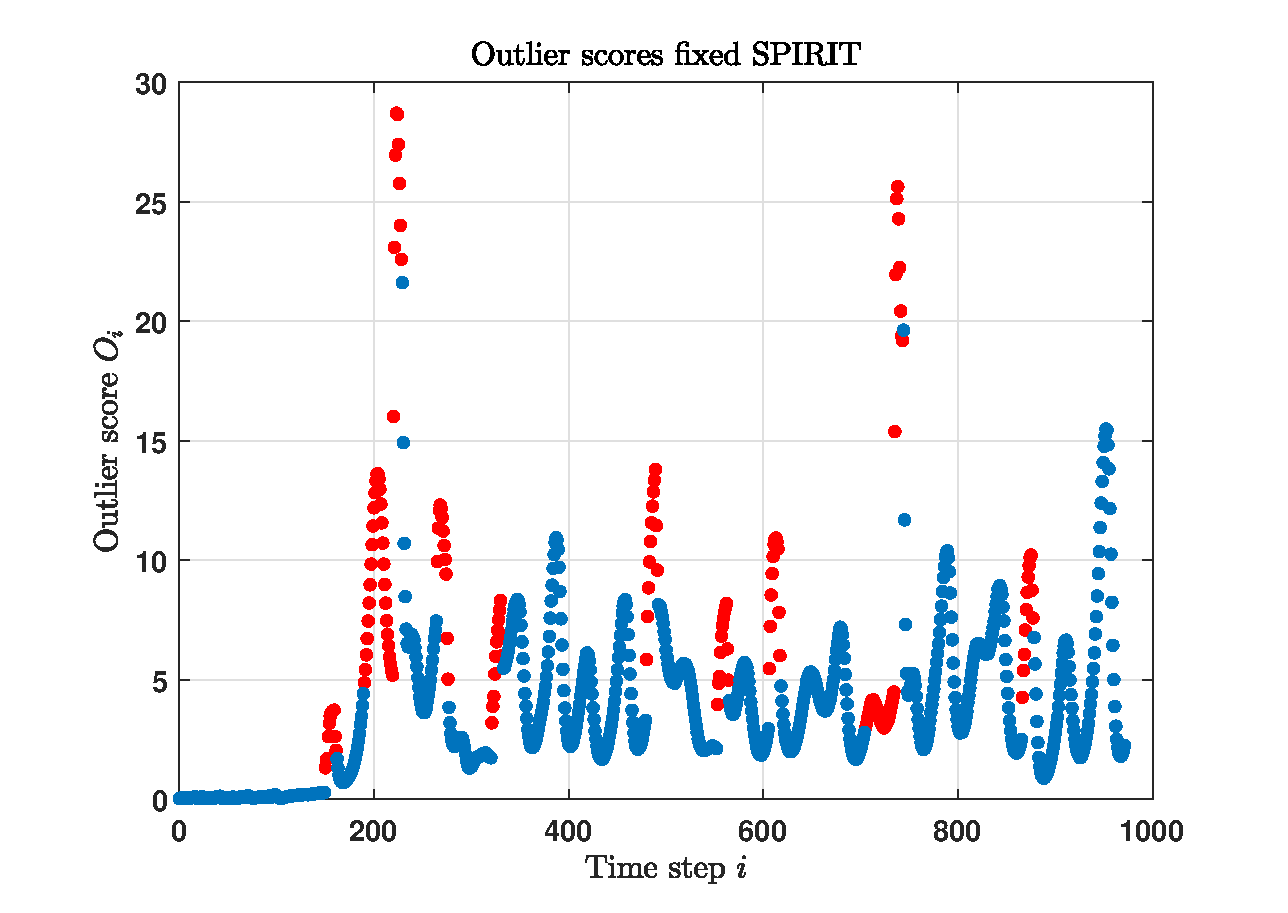
\includegraphics[scale=0.3]{parti/Outlierscores_fixedSPIRIT}
	\label{fig:parti_outlierscores_fixedspirit}
	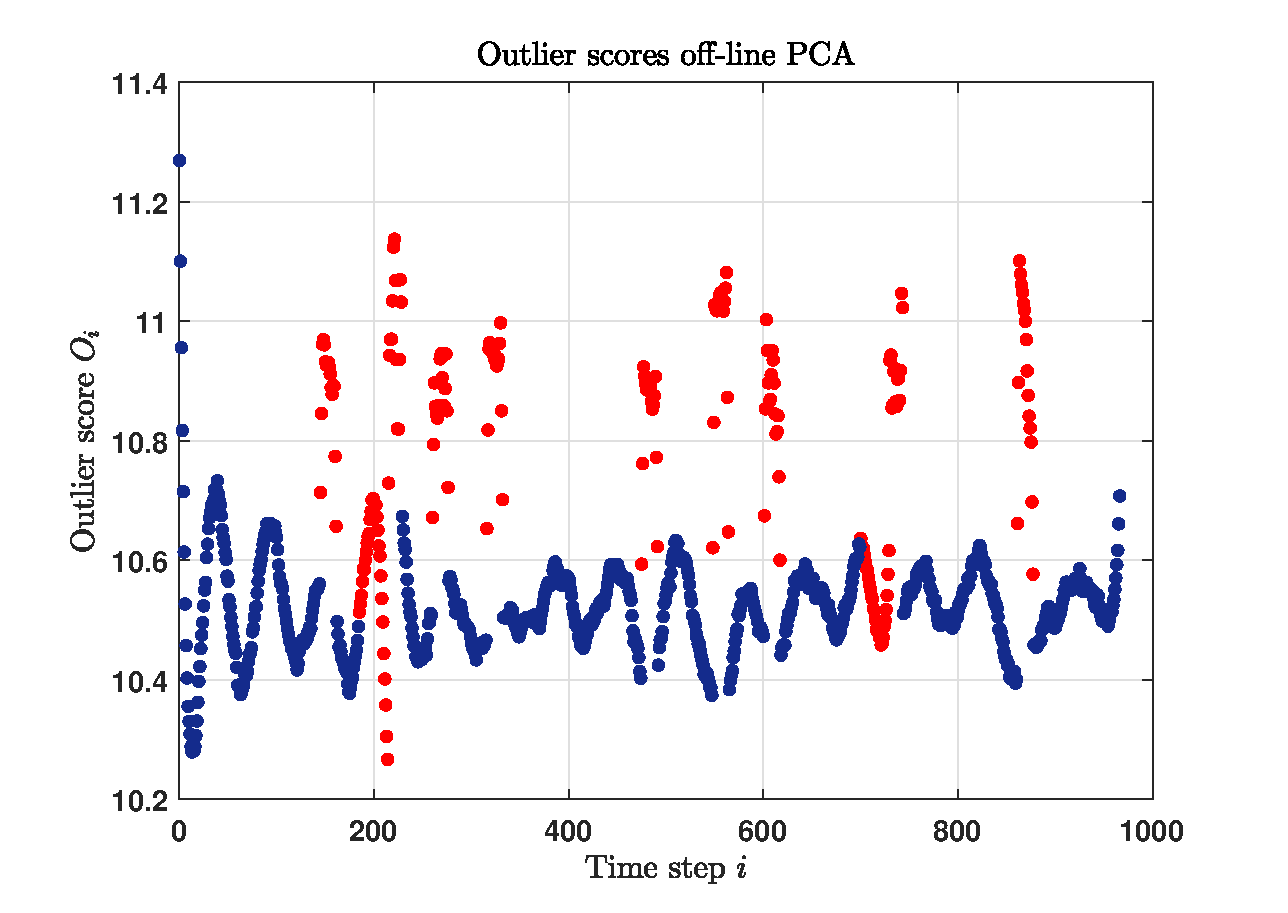
\includegraphics[scale=0.3]{parti/Outlierscores_PCA}
	\label{fig:parti_outlierscores_pca}
	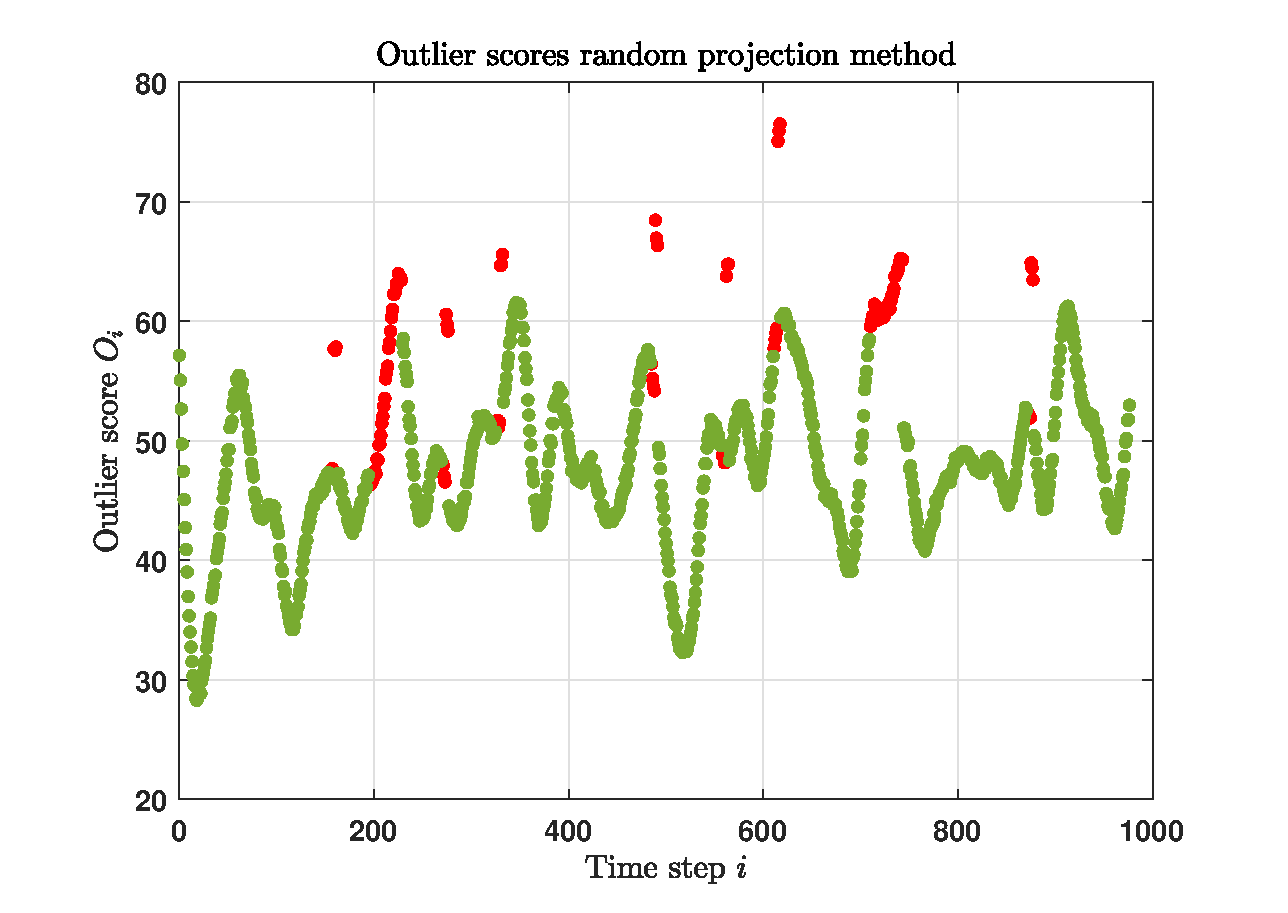
\includegraphics[scale=0.3]{parti/Outlierscores_RP}
	\label{fig:parti_outlierscores_rp}
	\caption{Outlier scores as resulting from the random projection method (\ref{fig:parti_outlierscores_rp}), the adaptive SPIRIT method (\ref{fig:parti_outlierscores_adaptivespirit}), the fixed SPIRIT method (\ref{fig:parti_outlierscores_fixedspirit}) and off-line PCA (\ref{fig:parti_outlierscores_pca}).}
	\label{fig:parti_outlierscores}
\end{figure}


It turns out that the RP method is sufficiently `bad' at modelling the outliers, such that the reconstruction error indeed shows a higher deviation for those data points. However, the reconstruction errors from the random projections still show the behaviour of the sinusoidal function which indicates the preference for an adaptive threshold to filter out the false positives. This can be derived from the ROC curves in figure \ref{fig:parti_rocs}, SPIRIT with a fixed number of components shows a steep ROC curve at the start but it does not succeed in finding most of the data points belonging to the class of outliers. That is, it reaches a $TPR$ of 0.67 while misclassifying around 10 percent ($FPR\approx0.1$) of the normal data points. The random projection method however succeed in finding 90 percent of the outliers, but at the cost of labelling 20 percent of the normal data points as outliers as well.

[Also explain that looking at these specific outlier scores, all methods label at least one 'data point' or window (out of 3 for point, or 15?20? for sequential) to incorporate an outlier, which might nuance the lower AUC scores. 
The window size also affects the detection time as we are being delayed if we take a larger window length]\\



Despite the desire to provide a summarizing overview with explicit quantized performance results, and a definite judgement about the method that is concluded to be the most promising given the analyses. However, as we are practising outlier detection in an unsupervised context, it might be better to conclude with a qualitative comparison instead. To that end, table \ref{tab:parti_qualcomp} provides the final judgement.

\begin{table}
	\caption{Qualitative comparison between proposed method and baseline}
	\label{tab:parti_qualcomp}
	\begin{tabular}{l c c c c c }
		\toprule
		Method & Detection performance & Runtime performance & Memory & Stability & Sensitivity \\\midrule
		SPIRIT 				&	+	&	-	&	- 	& + & - \\
		Random projections 	&	+	&	+	&	+	& - & + \\
		\bottomrule
	\end{tabular}
\end{table}


\section{Reducing instability}
RP method for some data sets might be uncertain as indicated by the relatively high standard deviation. In such cases it seems useful to take use an ensemble of multiple predictions obtained by several distinct random projection matrices. If we take 8 distinct runs with the reconstruction-based outlier detection method using random projections, we see that the standard deviation is reduced significantly, where also the average is increased a little. Table \ref{tab:parti_characteristics1}.

\begin{table}[h]
	\centering
	\caption{Performance basic random projection method and an ensemble version}
	\label{tab:parti_characteristics1}
	\begin{tabular}{l c c}
		\toprule	
		Method					&	AUC	& Runtime\\
		\midrule
		Random projections		& 0.928 ($\pm$ 0.01) & 0.024 ($\pm$ 0.004)\\
		Random projections ensemble	& \textbf{0.929 ($\pm$ 0.0004)} & 0.13 ($\pm$ 0.07)\\
		\bottomrule
	\end{tabular}
\end{table}



\section{Concluding remarks}
\label{sec:parti_concluding}

[Just one vector as projection...]

[- Distributing is not expected to improve as the reconstruction-based method does not have the benefit of preserving distances. To that end, there is no incentive to compensate for the probability we obtain a representation of the data that is not of high quality in the sense that our distances are being preserved. Also, as we have seen in this chapter, the standard deviation of the AUCs were very small, and we do not benefit much from using a high number of projection vectors.... The RP theory states we attain a distance preserving representation with a certain high probability, which is most beneficial for our feature reduction method.]\\

Methods based on principal component analysis benefit from larger windows, i.e. it benefits from having more historic information from a certain time series at each time step. The random projection method however does not. Another remarkable finding is that the rule `less is more' seems to apply to the random projection method, which was not expected on forehand. The intuition we have at this moment, is that even if your projection is very badly functioning as a reconstruction based, it still reconstructs outliers worse than it reconstructs normal data points.\\

Using random projections for reconstruction-based outlier detection seems a very promising method. We would like to note that its success stands or falls with the scaling of the projection matrix $\bf{R}$ and the projected vectors $\bf{x}'$. In case we focus on class separability, preserving the original distances might not make a difference, as was pointed out in \cite{fradkin2003experiments}. However, in this chapter we have identified a high impact of the different scaling methods even when classification relies on Euclidean distances.\\

The performances over the ROCs are investigated as no thresholding method is implemented. It is likely that thresholding approaches come close to the optimal operating window, but the optimal point is hard to reach with a certain fixed thresholding method. However, as the outlier scores of the random projections do not capture the principal behaviour, it would be better to adopt an adaptive thresholding scheme like the one discussed in  (Cite on-line adaptive thresholding).\\

As reflected by the ROC curves in figure \ref{fig:parti_rocs} and the outlier scores in figure \ref{fig:parti_outlierscores_rp}, the reconstruction from random projections results in many false positives as it does not capture the principal behaviour of the time series. What also becomes clear, is that methods based on principal components analysis suffer from the high dimensional data.% WHY
Regardless of that, it seems well (and better) capable of not misclassifying normal data points as being outliers. That makes us question: can we make the life of principal component analysis based methods easier, and even better? Our hypothesis is that we can do this, if we combine the two forces and deploy random projections in a different way which will be further investigated in \ref{chap:partii}.



